\documentclass[11pt, oneside]{article}
\usepackage[letterpaper, margin=2cm]{geometry}
\usepackage{MATH565}

\begin{document}
\noindent \textbf{\Large{Caleb Logemann \\
MATH 565 Continuous Optimization \\
Homework 2
}}

%\lstinputlisting[language=Python]{H01_23.m}
\begin{enumerate}
  \item % #1
    Problem 6 \\
    Consider the steepest descent method with exact linear searches applied to
    the convex quadractic function (3.24).
    Using the properties given in this chapter, show that if the initial point
    is such that $x_0 - x^*$ is parallel to an eigenvector of $Q$, then the
    steepest descent method will find the solution in one step.

    \begin{proof}
      We are considering applying the steepest descent method to the function
      \[
        f(\v{x}) = \frac{1}{2} \v{x}^T\M{Q}\v{x} - \v{b}^T \v{x}.
      \]
      Also the initial point $\v{x}_0$ satisfies $\v{x}_0 - \v{x}^*$ being parallel to an
      eigenvector of $\M{Q}$.
      This implies that $\v{x}_0 - \v{x}^*$ is an eigenvector of $Q$, so let
      $\lambda$ denote the eigenvalue associated with this eigenvector.

      The steepest descent method uses the following search direction
      \[
        p_0 = -\nabla f(x_0)
      \]
      Since
      \[
        \nabla f(x) = \M{Q} \v{x} - \v{b}
      \]
      the initial search direction will be
      \[
        p_0 = -\p{\M{Q}\v{x}_0 - \v{b}}
      \]
      This can be simplified by noticing that $x^*$ the minimizer of $f$ is the
      point that satisfies $\nabla f(x^*) = 0$ because $f$ is convex.
      This can be solved as follows.
      \begin{align*}
        \nabla f(x^*) &= 0 \\
        \M{Q}\v{x}^* - \v{b} &= 0 \\
        \M{Q}\v{x}^* &= \v{b} \\
        \v{x}^* &= \M{Q}^{-1}\v{b}
      \end{align*}
      The inverse of $\M{Q}$ exists because $Q$ is symmetric positive definite.
      Using this we can simplify $p_0$.
      \begin{align*}
        \v{p}_0 &= -\p{\M{Q}\v{x}_0 - \v{b}} \\
        \v{p}_0 &= -\p{\M{Q}\v{x}_0 - \M{Q}\M{Q}^{-1}\v{b}} \\
        \v{p}_0 &= -\M{Q}\p{\v{x}_0 - \M{Q}^{-1}\v{b}} \\
        \v{p}_0 &= -\M{Q}\p{\v{x}_0 - \v{x}^*}
        \intertext{Since $\v{x}_0 - \v{x}^*$ is an eigenvector of $Q$.}
        \v{p}_0 &= -\lambda\p{\v{x}_0 - \v{x}^*}
      \end{align*}

      Now that the search direction has been specified the step size must be
      determined.
      When using an exact line search the solution of the following minimization
      problem must be determined.
      \[
        \min[\alpha > 0]{f(\v{x}_0 + \alpha \v{p}_0)} = \min[\alpha > 0]{\phi(\alpha)}
      \]
      The function $\phi(\alpha)$ can be simplified as follows.
      \begin{align*}
        \phi(\alpha) &= f(x_0 + \alpha p_0) \\
        &= \frac{1}{2}\p{\v{x}_0 + \alpha \v{p}_0}^T \M{Q} \p{\v{x}_0 + \alpha \v{p}_0} - \v{b}^T \p{\v{x}_0 + \alpha \v{p}_0} \\
        &= \frac{1}{2}\p{\v{x}_0^T \M{Q} \v{x}_0 + \alpha \v{x}_0^T \M{Q} \v{p}_0 + \alpha \v{p}_0^T \M{Q} \v{x}_0 + \alpha^2 \v{p}_0^T \M{Q} \v{p}_0} - \v{b}^T \v{x}_0 - \alpha \v{b}^T \v{p}_0
        \intertext{Since $\M{Q}$ is symmetric}
        &= \frac{1}{2}\p{\v{x}_0^T \M{Q} \v{x}_0 + 2 \alpha \v{x}_0^T \M{Q} \v{p}_0 + \alpha^2 \v{p}_0^T \M{Q} \v{p}_0} - \v{b}^T \v{x}_0 - \alpha \v{b}^T \v{p}_0 \\
        &= \p{\frac{1}{2} \v{p}_0^T \M{Q} \v{p}_0} \alpha^2 + \p{\v{x}_0^T \M{Q} \v{p}_0 - \v{b}^T \v{p}_0} \alpha + \v{x}_0^T \M{Q} \v{x}_0 - \v{b}^T \v{x}_0
      \end{align*}
      In order to minimize this function we must differentiate with respect to
      $\alpha$ and set equal to zero.
      \begin{align*}
        \phi'(\alpha) &= \v{p}_0^T \M{Q} \v{p}_0 \alpha + \p{\v{x}_0^T \M{Q} \v{p}_0 - \v{b}^T \v{p}_0} \\
        0 &= \v{p}_0^T \M{Q} \v{p}_0 \alpha + \p{\v{x}_0^T \M{Q} \v{p}_0 - \v{b}^T \v{p}_0} \\
        \alpha &= \frac{\v{b}^T \v{p}_0 - \v{x}_0^T \M{Q} \v{p}_0}{\v{p}_0^T \M{Q} \v{p}_0}
        \intertext{This can be simplified by plugging in the value of $\v{p}_0$}
        \alpha &= \frac{\lambda \v{b}^T\p{\v{x}_0 - \v{x}^*} - \lambda \v{x}_0^T \M{Q} \p{\v{x}_0 - \v{x}^*}}{\lambda^2 \p{\v{x}_0 - \v{x}^*}^T\M{Q} \p{\v{x}_0 - \v{x}^*}}
        \intertext{Since $\v{x}_0 - \v{x}^*$ is an eigenvector of $\M{Q}$.}
        \alpha &= \frac{\lambda \v{b}^T\p{\v{x}_0 - \v{x}^*} - \lambda^2 \v{x}_0^T \p{\v{x}_0 - \v{x}^*}}{\lambda^3 \p{\v{x}_0 - \v{x}^*}^T\p{\v{x}_0 - \v{x}^*}} \\
        \alpha &= \frac{\lambda \v{b}^T\p{\v{x}_0 - \v{x}^*} - \lambda^2 \v{x}_0^T \p{\v{x}_0 - \v{x}^*}}{\lambda^3 \norm{\v{x}_0 - \v{x}^*}^2}
      \end{align*}
    \end{proof}

  \item % #2
    Problem 8 \\
    Let $Q$ be a postive definite symmetric matrix.
    Prove that for any vector $\v{X}$, we have
    \[
      \frac{\p{\v{x}^T\v{x}}^2}{\p{\v{x}^T \M{Q} \v{x}}\p{\v{x}^T \M{Q}^{-1} \v{x}}}
      \ge \frac{4\lambda_n \lambda_1}{\p{\lambda_n + \lambda_1}^2}
    \]
    where $\lambda_n$ and $\lambda_1$ are, respectively, the largest and
    smallest eigenvalues of $\M{Q}$.
    (This relation, which is known as the Kantorovich inequality, can be used to
    deduce (3.29) from (3.28).)

  \item % #3 Done
    Problem 12 \\
    Consider a block diagonal matrix $\M{B}$ with $1 \times 1$ and $2 \times 2$
    blocks.
    Show that the eigenvalues and eigenvectors can be obtained by computing the
    spectral decomposition of each block separately.

    \begin{proof}
      Let $\M{B}$ be block diagonal and let $\M{B}_k$ be the blocks along the diagonal.
      Let $n$ be the total number of blocks.
      Each block can be written as its spectral decomposition, that is
      \[
        \M{B}_k = \M{Q}_k \M{\Lambda}_k \M{Q}_k^{-1}
      \]
      where $\Lambda_k$ is a diagonal matrix of the eigenvalues of $B_k$ and
      $\M{Q}_k$ and $\M{Q}_k^{-1}$ are the left and right eigenvectors
      respectively.
      Using these spectral decompositions we can create the spectral
      decomposition of $\M{B}$.
      Let $\M{\Lambda}$ be a block diagonal matrix of all the $\M{\Lambda}_k$
      matrices.
      Note that since the $\M{\Lambda}_k's$ are diagonal this means that
      $\M{\Lambda}$ will be diagonal not just block diagonal.
      Also let $\M{Q}$ be a block diagonal matrix of the $\M{Q}_k$ matrices.
      If this is the case then $\M{Q}^{-1}$ will be a block diagonal matrix
      of the matrices $\M{Q}_k^{-1}$.
      Visually these matrices are
      \begin{align*}
        \M{\Lambda} &=
        \begin{bmatrix}
          \M{\Lambda}_1 & & & \\
          & \M{\Lambda}_2 & & \\
          & & \ddots & \\
          & & & \M{\Lambda}_n \\
        \end{bmatrix} \\
        \M{Q} &=
        \begin{bmatrix}
          \M{Q}_1 & & & \\
          & \M{Q}_2 & & \\
          & & \ddots & \\
          & & & \M{Q}_n \\
        \end{bmatrix} \\
      \end{align*}
      To verify that $\M{B} = \M{Q} \M{\Lambda} \M{Q}^{-1}$ is indeed the
      spectral decomposition of $\M{B}$ will multiply these three matrices out.
      \begin{align*}
        \M{Q} \M{\Lambda} \M{Q}^{-1} &= 
        \begin{bmatrix}
          \M{Q}_1 & & & \\
          & \M{Q}_2 & & \\
          & & \ddots & \\
          & & & \M{Q}_n
        \end{bmatrix}
        \begin{bmatrix}
          \M{\Lambda}_1 & & & \\
          & \M{\Lambda}_2 & & \\
          & & \ddots & \\
          & & & \M{\Lambda}_n
        \end{bmatrix}
        \begin{bmatrix}
          \M{Q}_1^{-1} & & & \\
          & \M{Q}_2^{-1} & & \\
          & & \ddots & \\
          & & & \M{Q}_n^{-1}
        \end{bmatrix} \\
        &=
        \begin{bmatrix}
          \M{Q}_1 \M{\Lambda}_1 \M{Q}_1^{-1}& & & \\
          & \M{Q}_2 \M{\Lambda}_2 \M{Q}_2^{-1}& & \\
          & & \ddots & \\
          & & & \M{Q}_n\M{\Lambda}_n\M{Q}_n^{-1}
        \end{bmatrix} \\
        &=
        \begin{bmatrix}
          \M{B}_1 & & & \\
          & \M{B}_2 & & \\
          & & \ddots & \\
          & & & \M{B}_n
        \end{bmatrix} \\
        &= \M{B}
      \end{align*}
      This shows that the eigenvalues of $\M{B}$ are the union of the eigenvalues
      of the matrices $\M{B}_k$.
      Also the eigenvectors of $\M{B}$ are related to the eigenvectors of
      $\M{B}$.
      The eigenvectors of $\M{B}$ are the columns of $\M{Q}$, so they are the
      eigenvectors of $\M{B}_k$ but embedded in zeroes in the proper way.
    \end{proof}

  \item % #4 Done
    For the quadractic function
    \[
      f(\v{x}) = \frac{1}{2} \v{x}^T \M{B} \v{x} - \v{x}^T \v{b}
    \]
    where $\M{B} \in \RR^{n \times n}$ is symmetric positive definite, show that
    the Newton search direction with $\alpha = 1$ satisfies the sufficient
    decrease assumption (3.4) for any $c_1 \le \frac{1}{2}$ and the curvature
    conditions (3.5) for any $c_2 > 0$.

    \begin{proof}
      For Newton's method the search direction is
      \[
        \v{p}_k = -\nabla^2 f(\v{x}_k)^{-1} \nabla f(\v{x}_k)
      \]
      For the given function we can find formulas for the gradient and Hessian.
      \begin{align*}
        \nabla f(\v{x}) &= \M{B} \v{x} - \v{b} \\
        \nabla^2 f(\v{x}) &= \M{B} \\
      \end{align*}
      Plugging this in to the search direction we find that
      \begin{align*}
        \v{p}_k &= - \M{B}^{-1} \p{\M{B} \v{x}_k - \v{b}} \\
        &= -\v{x}_k + \M{B}^{-1} \v{b}
      \end{align*}
      Since $\alpha = 1$, $\v{x}_k + \alpha \v{p}_k$ can be simplified.
      \begin{align*}
        \v{x}_k + \alpha \v{p}_k &= \v{x}_k + \v{p}_k \\
        &= \v{x}_k - \v{x}_k + \M{B}^{-1} \v{b} \\
        &= \M{B}^{-1} \v{b}
      \end{align*}
      The last expression that is useful to simplify is $\nabla f(x_k)^T \v{p}_k$.
      \begin{align*}
        \nabla f(\v{x}_k)^T \v{p}_k &= \p{\M{B} \v{x}_k - \v{b}}^T \p{\M{B}^{-1} \v{b} - \v{x}_k} \\
        \intertext{Because $\M{B}$ is symmetric $\M{B}^T = \M{B}$}
        &= \p{\v{x}_k^T \M{B} - \v{b}^T} \p{\M{B}^{-1} \v{b} - \v{x}_k} \\
        &= \v{x}_k^T \M{B} \M{B}^{-1} \v{b} - \v{x}_k^T \M{B} \v{x}_k - \v{b}^T \M{B}^{-1} \v{b} + \v{b}^T\v{x}_k \\
        &= \v{x}_k^T \v{b} - \v{x}_k^T \M{B} \v{x}_k - \v{b}^T \M{B}^{-1} \v{b} + \v{x}_k^T \v{b} \\
        &= 2\v{x}_k^T \v{b} - \v{x}_k^T \M{B} \v{x}_k - \v{b}^T \M{B}^{-1} \v{b} \\
      \end{align*}

      Using these expressions I will verify both conditions.
      First the sufficient decrease condition states that
      \[
        f(\v{x}_k + \alpha p_k) \le f(\v{x}_k) + c_1 \alpha \nabla f_k^T \v{p}_k
      \]
      The left hand side is
      \begin{align*}
        f(\v{x}_k + \alpha p_k) &= f(\M{B}^{-1} \v{b}) \\
        &= \frac{1}{2} (\M{B}^{-1} \v{b})^T \M{B} \M{B}^{-1} \v{b} - (\M{B}^{-1} \v{b})^T \v{b} \\
        \intertext{The inverse of $B$ is also symmetric}
        &= \frac{1}{2} \v{b}^T \M{B}^{-1} \v{b} - \v{b}^T \M{B}^{-1} \v{b} \\
        &= -\frac{1}{2} \v{b}^T \M{B}^{-1} \v{b}
      \end{align*}
      The right hand side is
      \begin{align*}
        f(\v{x}_k) + c_1 \alpha \nabla f_k^T \v{p}_k &= \frac{1}{2}\v{x}_k^T \M{B} \v{x} - \v{x}_k^T \v{b} + c_1\p{2\v{x}_k^T \v{b} - \v{x}_k^T \M{B} \v{x}_k - \v{b}^T \M{B}^{-1} \v{b}} \\
        &=\p{\frac{1}{2} - c_1}\v{x}_k^T \M{B} \v{x} + \p{2c_1 - 1}\v{x}_k^T \v{b} + -c_1\v{b}^T \M{B}^{-1} \v{b}
      \end{align*}
      Note that $\p{\frac{1}{2} - c_1}\v{x}_k^T \M{B} \v{x}$ and $\p{2c_1 - 1}\v{x}_k^T \v{b}$
      are positive because $c_1 \le 1/2$ and $\M{B}$ is symmetric.
      This shows that
      \[
        -\frac{1}{2} \v{b}^T \M{B}^{-1} \v{b} \le \p{\frac{1}{2} - c_1}\v{x}_k^T \M{B} \v{x} + \p{2c_1 - 1}\v{x}_k^T \v{b} + -c_1\v{b}^T \M{B}^{-1} \v{b}
      \]
      which is equivalent to the sufficient decrease condition.

      Next I will show the curvature condition holds.
      \[
        \nabla f(x_k + \alpha p_k)^T \v{p}_k \ge c_2 \nabla f_k^T \v{p}_k
      \]
      The left hand side is
      \begin{align*}
        \nabla f(x_k + \alpha p_k)^T \v{p}_k &= \nabla f(\M{B}^{-1} \v{b})^T \p{\M{B}^{-1} \v{b} - \v{x}_k} \\
        &= \p{\M{B} \M{B}^{-1} \v{b} - \v{b}}^T \p{\M{B}^{-1} \v{b} - \v{x}_k} \\
        &= \v{0}^T \p{\M{B}^{-1} \v{b} - \v{x}_k} \\
        &= 0
      \end{align*}
      The right hand side is
      \begin{align*}
        c_2 \nabla f_k^T \v{p}_k &= c_2\p{2\v{x}_k^T \v{b} - \v{x}_k^T \M{B} \v{x}_k - \v{b}^T \M{B}^{-1} \v{b}} \\
      \end{align*}
      Both $\v{x}_k^T \M{B} \v{x}_k$ and $\v{b}^T \M{B}^{-1} \v{b}$ are
      positive as $B$ is positive definite.
      Also $\v{x}_k^T \M{B} \v{x}_k \ge \norm{\v{x}_k}$ and $\v{b}^T \M{B}^{-1} \v{b} \ge \norm{\v{b}}$.
      This with the fact that $\v{x}_k^T \v{b} \le \norm{\v{x}} + \norm{\v{b}}$, gives
      \[
        c_2 \nabla f_k^T \v{p}_k \le 0 = \nabla f(x_k + \alpha p_k)^T \v{p}_k
      \]
      This shows that the curvature condition is met.
    \end{proof}

  \item % #5 Done
    Consider the function:
    \[
      f(\v{x}) = 20(x_2 - x_1^2)^2 + (1 - x_1)^2
    \]
    Write a \MATLAB steepest descent code to find the minimizer of this function.
    The function be in the form
    \begin{lstlisting}[language=MATLAB, frame=none]
      xstar = SteepestDescent(f, x0, TOL, MaxIters)
    \end{lstlisting}
    Use $\v{x_0} = (1.2, 1.2)^T$.
    Use an exact line search to find $\alpha$.
    You can use your $1D$ rootfinding code from Homework 1 to compute the exact
    line search solution $\alpha$.
    Plot the contour lines of $f$ and superimport the various guesses (each
    connected to the next via a line segment) made by the steepest descent
    algorithm.
    Produce a table of your approximations and the errors (if there are many
    iterations, you can just show the first 10 iterations and the last 10
    iterations).

    In order to compute the exact line search I implemented Newton's Method in
    one dimension to compute roots of $\d{\phi}{\alpha}$.
    Note that Newton's Method requires $\d[2]{\phi}{\alpha}$ as well.
    The other problem with this approach is that Newton's Method is only
    finding roots of $\d{\phi}{\alpha}$ and not finding the absolute minimum of
    $\phi(\alpha)$.
    It may in fact find only a local minimum or even a maximum.
    However this method is right most of the time and allows the Steepest Descent
    method to converge in this case.
    My implementation of Newton's Method in one dimension is shown below.
    \lstinputlisting[language=Python]{newton1D.py}
    The next script implements and uses the Steepest Descent algorithm to find
    the global minimum of $f$.
    \lstinputlisting[language=Python]{02_5.py}

    The following table lists the first 10 and last 10 approximations.
    The error in these tables is also the function values at the approximation
    as the minimum value is zero.
    \begin{center}
      \begin{tabular}{cccc}
        \toprule
        $k$ & $\p{x_1}_k$ & $\p{x_2}_k$ & $e_k$ \\
        \midrule
          0 & 1.2           & 1.2           & 1.19199999999e+00 \\
          1 & 1.11100773654 & 1.23644734339 & 1.24116880777e-02 \\
          2 & 1.06441606231 & 1.12268600547 & 6.26939535114e-03 \\
          3 & 1.05988566879 & 1.12454145675 & 3.61432219908e-03 \\
          4 & 1.04015601545 & 1.07636821985 & 2.22995866730e-03 \\
          5 & 1.03761784087 & 1.07740774527 & 1.42656176856e-03 \\
          6 & 1.02655884997 & 1.05040537581 & 9.38985518567e-04 \\
          7 & 1.02496393975 & 1.05105858136 & 6.28349485527e-04 \\
          8 & 1.01809348915 & 1.03428323113 & 4.26932414201e-04 \\
          9 & 1.01703824335 & 1.03471541371 & 2.92732528178e-04 \\
         10 & 1.01253992599 & 1.02373202217 & 2.02555033610e-04 \\
        \vdots & \vdots & \vdots & \vdots \\
        %116 & 1.00000000025 & 1.00000000047 & 7.92662519641e-20 \\
        117 & 1.00000000023 & 1.00000000047 & 5.68480731488e-20 \\
        118 & 1.00000000018 & 1.00000000033 & 4.07321772830e-20 \\
        119 & 1.00000000017 & 1.00000000034 & 2.91848895231e-20 \\
        120 & 1.00000000012 & 1.00000000024 & 2.09013306391e-20 \\
        121 & 1.00000000012 & 1.00000000024 & 1.49689263278e-20 \\
        122 & 1.00000000009 & 1.00000000017 & 1.07321945388e-20 \\
        123 & 1.00000000008 & 1.00000000017 & 7.69439383459e-21 \\
        124 & 1.00000000006 & 1.00000000012 & 5.52176221112e-21 \\
        125 & 1.00000000006 & 1.00000000012 & 3.96265903408e-21 \\
        126 & 1.00000000004 & 1.00000000008 & 2.84303547930e-21 \\
      \end{tabular}
    \end{center}
    The following contour plot was also produced.
    \begin{center}
      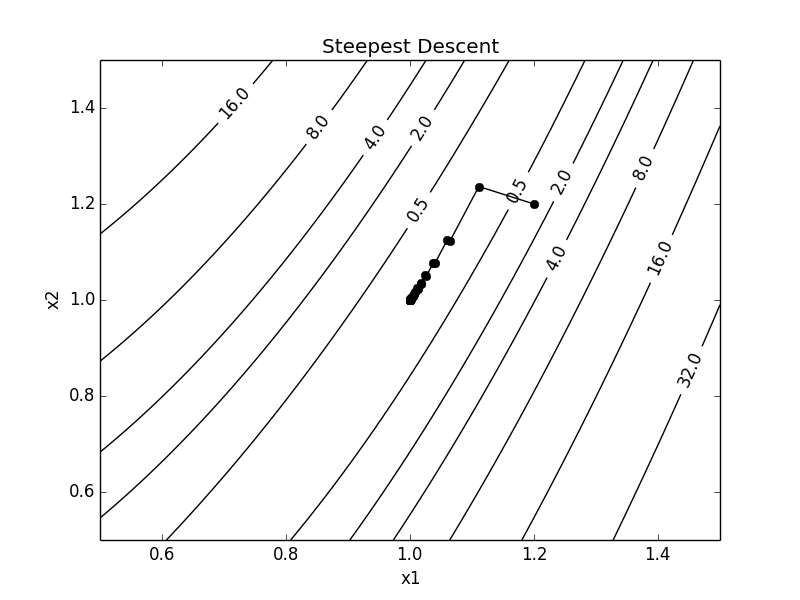
\includegraphics[scale=.5]{Figures/02_1}
    \end{center}

  \item % #6 Done
    Consider the function:
    \[
      f(\v{x}) = 20(x_2 - x_1^2)^2 + (1 - x_1)^2
    \]
    Write a \MATLAB Newton descent code to find the minimizer of this function.
    The function be in the form
    \begin{lstlisting}[language=MATLAB, frame=none]
      xstar = NewtonDescent(f, x0, TOL, MaxIters)
    \end{lstlisting}
    Use $\v{x_0} = (1.2, 1.2)^T$.
    Use $\alpha = 1$.
    Use the backslash operator to invert the appropriate matrices.
    Plot the contour lines of $f$ and superimport the various guesses (each
    connected to the next via a line segment) made by the Newton descent
    algorithm.
    Produce a table of your approximations and the errors (if there are many
    iterations, you can just show the first 10 iterations and the last 10
    iterations).

    The following script implements and runs Newton's Method in multi dimensions
    to find the minimum of $f$.
    Note that this script uses the plotResults function from the script in the
    previous problem.
    \lstinputlisting[language=Python, firstline=28]{02_6.py}
    The following table describes the list of approximations and errors.
    Note that the error at step $k$ is equal to the function value at
    $\p{x_1}_k$ and $\p{x_2}_k$, because the minimum value is zero.
    \begin{center}
      \begin{tabular}{cccc}
        \toprule
        $k$ & $\p{x_1}_k$ & $\p{x_2}_k$ & $e_k$ \\
        \midrule
        0 & 1.2            & 1.2           & 1.1919999999 \\
        1 & 1.181132075471 & 1.39471698113 & 3.2811363464e-02 \\
        2 & 1.002543096882 & 0.97319863783 & 2.0351041753e-02 \\
        3 & 1.001425625865 & 1.00285203539 & 2.0324402951e-06 \\
        4 & 1.000000071205 & 0.99999811020 & 8.2602301879e-11 \\
        5 & 1.000000000005 & 1.00000000001 & 3.3499320311e-23 \\
        \bottomrule
      \end{tabular}
    \end{center}
    The following contour plot was also produced.
    \begin{center}
      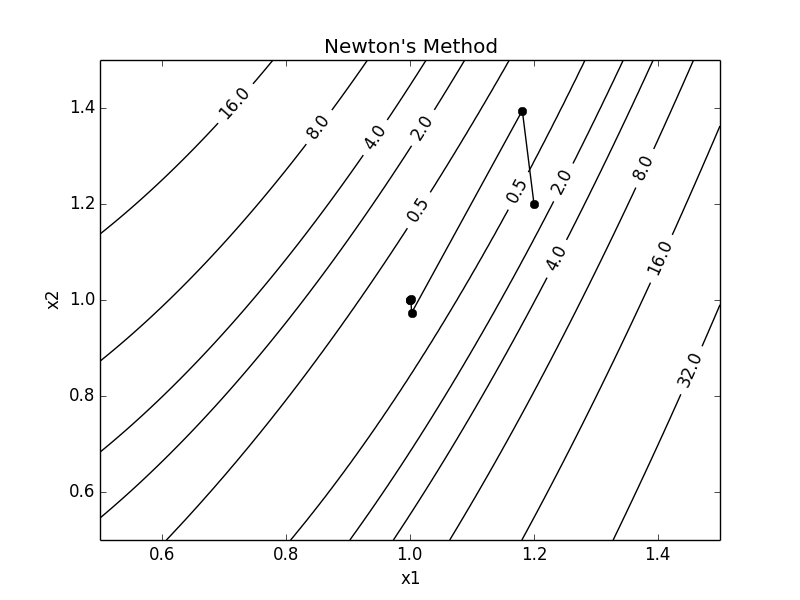
\includegraphics[scale=.5]{Figures/02_2}
    \end{center}

\end{enumerate}
\end{document}
